\section{Theorie}
\label{sec:Theorie}

Brückenschaltungen können jede physikalische Größe messen, welche eindeutig durch einen
elektrischen Widerstand darstellbar ist. In einer Brückenschaltung wird die Potentialdifferenz zweier elektrischer Leiter
in Abhängigkeit von ihrem Widerstandsverhältnis untersucht.


\begin{figure}[H]
  \centering
  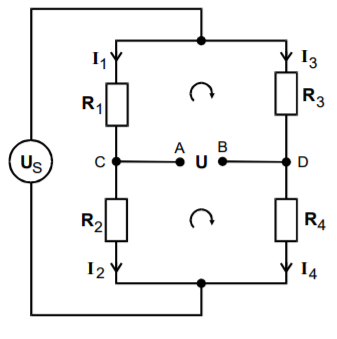
\includegraphics[height=5cm]{bruecke.PNG}
  \caption{Darstellung einer allgemeinen Brückenschaltung. \cite{sample}}
  \label{fig:Brückenschaltung}
\end{figure}

Mithilfe der beiden Kirchhoffschen Gesetze lässt sich die Spannung $U$ der Brückenschaltung wie folgt darstellen.
\begin{equation}
  U = \frac{R_2 R_3 - R_1 R_4}{(R_3+R_4)(R_1+R_2)}U_S
\end{equation}

Dabei ist $U_S$ die Speisespannung. Für den Fall $R_2R_3=R_1R_4$ verschwindet die gemessene Spannung, wodurch der Fall
der abgeglichene Brücke vorliegt. Ist $R_1$ ein unbekannter Widerstand, kann dieser durch das variieren der anderen Widerstände bestimmt werden,
indem untersucht wird, wann die Spannung verschwindet.

Sind die Widerstände komplex, also $R= X + jY$, so müssen zwei Bedingungen gleichzeitig erfüllt sein:
\begin{align}
  X_1X_4 -Y_1Y_4 &= X_2X_3 - Y_2Y_3 \\
  X_1Y_4 +X_4Y_1 &= X_2Y_3 + X_3Y_2
\end{align}


Im folgenden werden verschiedene
Brückenschaltungen beschrieben, welche die für diesen Versuch gesuchten Größen ermitteln.

\subsection{Wheatstonesche Brücke}
Die Wheatstonesche Brückenschaltung besteht aus vier Widerständen.

\begin{figure}[H]
  \centering
  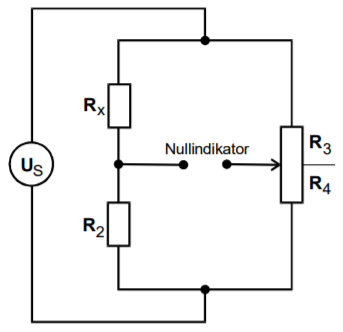
\includegraphics[height=5cm]{wheat.PNG}
  \caption{Darstellung einer Wheatstoneschen Brückenschaltung. \cite{sample}}
  \label{fig:Wheat}
\end{figure}

Für den unbekannten Widerstand $R_x$ gilt die Abgleichbedingung:
\begin{equation}
  R_x = R_2 \frac{R_3}{R_4}
\end{equation}

\subsection{Kapazitätsmessbrücke}
Mit dieser Schaltung werden Kapazitäten bestimmt, weshalb mit komplexen Widerständen gerechnet werden muss.

\begin{figure}[H]
  \centering
  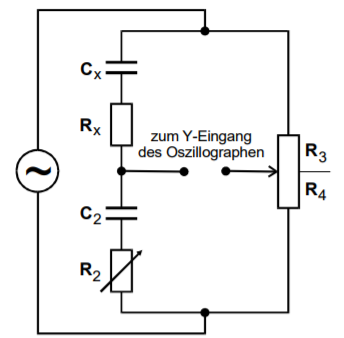
\includegraphics[height=5cm]{kapazitaet.PNG}
  \caption{Darstellung einer Kapazitätsmessbrücke. \cite{sample}}
  \label{fig:kapazität}
\end{figure}

Jeder  reale Kondensator besitzt einen Widerstand, welcher auch in Abbildung 3 dargestellt wird.
Der Widerstand eines Kondensators ist:
\begin{equation}
  R_{C_{real}} = R - \frac{j}{\omega C}
\end{equation}

Die unbekannten Größen $C_x$ und $R_x$ betragen:
\begin{align}
  C_x &= C_2 \frac{R_4}{R_3} \\
  R_x &= R_2 \frac{R_3}{R_4}
\end{align}

Für Frequenzen in dem Bereich von $10^4$Hz und kleiner gilt $R_2 \approx 0$.


\subsection{Induktivitätsmessbrücke}
Der komplexe Widerstand einer realen Spule ist definiert durch:
\begin{equation}
  R_{L_{real}} = R - j \omega L
\end{equation}

Die Induktivitätsmessbrücke ist analog zur Kapazitätsmessbrücke aufgebaut.

\begin{figure}[H]
  \centering
  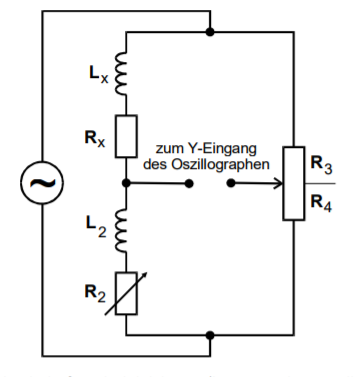
\includegraphics[height=5cm]{induktivitaet.PNG}
  \caption{Darstellung einer Induktivitätsmessbrücke. \cite{sample}}
  \label{fig:induktivitaet}
\end{figure}

Die Abgleichbedingungen sind:

\begin{align}
  L_x &= L_2 \frac{R_3}{R_4} \\
  R_x &= R_2 \frac{R_3}{R_4}
\end{align}

Damit diese Schaltung präzise Werte misst, muss die Spule einen möglichst kleinen Widerstand haben, für kleine Frequenzen
ist dieser dennoch zu groß, weshalb in diesem Fall die Maxwell-Brücke verwendet wird.

\subsection{Maxwell-Brücke}

\begin{figure}[H]
  \centering
  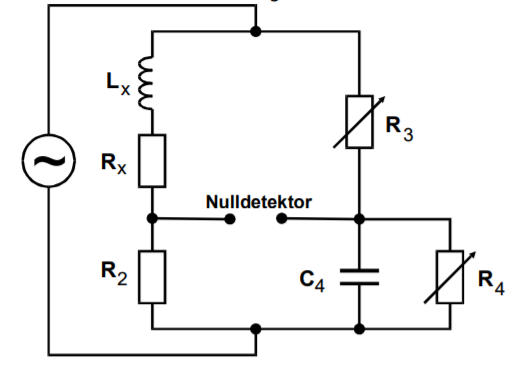
\includegraphics[height=5cm]{maxwell.PNG}
  \caption{Darstellung einer Maxwell-Brücke. \cite{sample}}
  \label{fig:maxwell}
\end{figure}

Der Widerstand $R_2$ soll dabei bekannt sein und als Abgleichelement dienen $R_3$ und $R_4$.
Für $L_x$ und $R_x$ ergibt sich dann:
\begin{align}
  L_x &= R_2 R_3 C_4 \\
  R_x &= \frac{R_2 R_3}{R_4}
\end{align}


\subsection{Wien-Robinson-Brücke}
Prinzipiell lassen sich Brückenschaltungen bei allen Frequenzen abgleichen. Es gibt jedoch einen
Frequenzbereich in dem ein Abgleich unter optimalen Bedingungen durchgeführt werden kann. Mit der
Wien-Robinson-Brücke soll dieser Bereich untersucht werden.

\begin{figure}[H]
  \centering
  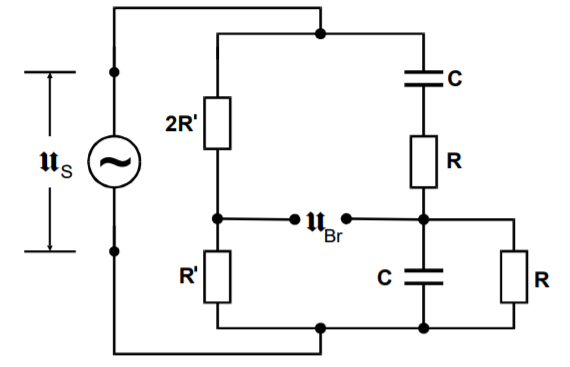
\includegraphics[height=5cm]{wien.PNG}
  \caption{Darstellung einer Wien-Robinson-Brücke. \cite{sample}}
  \label{fig:wien}
\end{figure}
Der Kondensator sollte in dieser Schaltung möglichst geringe Verluste besitzen.

Für das Betragsquadrat des Verhältnisses von der Brückenspannung $U_{Br}$ und der Speisespannung $U_S$ folgt:
\begin{equation}
  \left|\frac{U_{Br}}{U_S} \right|^2 = \frac{(\omega^2 R^2 C^2 -1)^2}{9((1- \omega^2 R^2 C^2) + 9 \omega^2 R^2 C^2)}
\end{equation}

Das Frequenzverhältnis $\Omega = \frac{\omega}{\omega_0}$ wird eingeführt. Dabei gilt:
\begin{equation}
  \omega_0 = \frac{1}{RC}
\end{equation}

Die Brückenspannung verschwindet bei der Frequenzt $\omega_0$.

Dann folgt aus Gleichung (13):
\begin{equation}
  \left|\frac{U_{Br}}{U_S} \right|^2 = \frac{1}{9} \frac{(\Omega^2 -1)^2}{(1- \Omega^2)^2 + 9 \Omega^2}
\end{equation}

Gleichung (15) hat die Form eines Filters. Die Wien-Robinson-Brücke schwächt Schwingungen in einem
Bereich um $\omega_0$ ab. Mit dieser Schaltung wird der Klirr-Faktor gemessen. Ein Sinusgenerator kann keine
Sinuschwingungen ohne Oberwellen erzeugen. Eine ideale Sinusschwingung besteht nur aus einer Grundschwingung.
Der Klirr-Faktor ist ein Maß für die Qualität des Sinusgenerators. Hat der Sinusgenerator die Sperrfrequenz $\omega_0$
der Wien-Robinson-Brücke, bleiben an dem Ausgang nur noch die Oberwellen. Die Summe deren Amplituden wird mit einem
Breitband-Millivoltmeter gemessen. Der Klirr-Faktor $k$ lässt sich mit Gleichung (16) berechnen, wobei nur die zweite
Oberwelle betrachtet wird:

\begin{equation}
  k = \frac{{U_2}}{U_1}
\end{equation}

Dabei ist $U_1$ die Grundschwingung und $U_2$ die erste Oberschwingung. Die erste Oberschwingung lässt sich wie folgt
berechnen:
\begin{equation}
  U_2 = \frac{U_{Br}}{f(2)}
\end{equation}


Die Funktion $f(2)$ ist Gleichung (15) mit $\Omega = 2$.
